\documentclass[10pt]{article}
\usepackage[margin=1in]{geometry}
\usepackage{graphicx}
\usepackage{float}
\begin{document}
	\begin{center}
			Colin Samplawski \\
			CS 760 - Homework 2
	\end{center}
\section*{Part 1}
See included code.
\section*{Part 2}
\begin{figure}[H]
\begin{minipage}[b]{0.49\textwidth}
	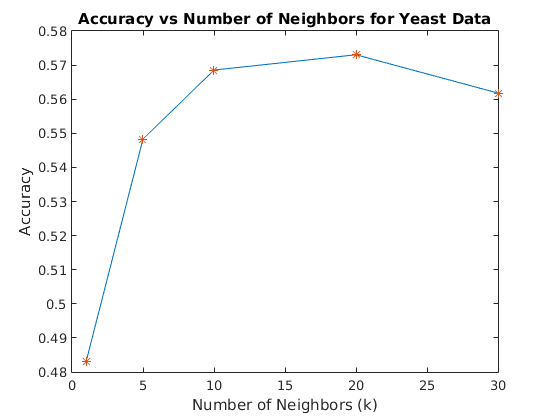
\includegraphics[width=\textwidth]{y_graph.jpg}
\end{minipage}
\hfill
\begin{minipage}[b]{0.49\textwidth}
	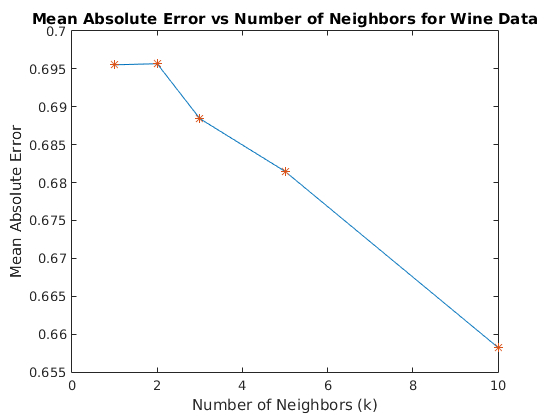
\includegraphics[width=\textwidth]{w_graph.jpg}
\end{minipage}
\end{figure}
\begin{figure}[H]
	\centering
	\begin{minipage}[b]{0.49\textwidth}
		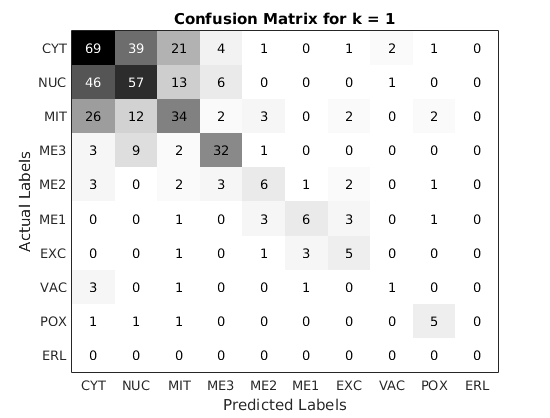
\includegraphics[width=\textwidth]{cmat_k1.jpg}
	\end{minipage}
	\hfill
	\begin{minipage}[b]{0.49\textwidth}
		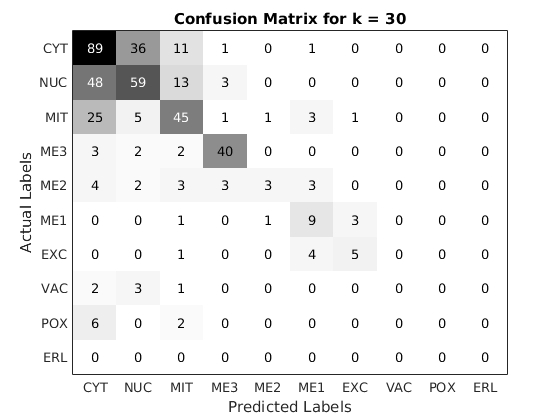
\includegraphics[width=\textwidth]{cmat_k30.jpg}
	\end{minipage}
\end{figure}
It easy to see that with using $k = 30$, there is less misclassified instances overall. This is not surprising given the graph above. It seems that most of the gains in accuracy where found in the better classification of instances with the CYT label, which is one of the more common labels in this data set. In fact, some other labels saw worse classification, such as NUC and MIT, but the gains in CYT compensated for it. Another interesting aspect of this data is that no testing instances had the ERL label and no instance was classified as such.

\section*{Part 3}
\begin{center}
\begin{tabular}{c| c |c |c |c}
	\hline
	operation & dist at this step & best dist & best node & queue \\ 
	\hline \hline 
	init & N/A & $\infty$ & N/A &  $(f,0)$ \\\hline
	pop $f$ & 7.071 & 7.071 & $f$ & $(h,0),(c,1)$ \\\hline
	pop $h$ & 7.071 & 7.071 & $f$ & $(i,0),(c,1),(g,5)$ \\\hline
	pop $i$ & 3 & 3 & $i$ & $(c,1),(j,3),(g,5)$ \\\hline
	pop $c$ & 2 & 2 & $c$ & $(b,0),(e,0),(j,3),(g,5)$ \\\hline
	pop $b$ & 4.472 & 2 & $c$ & $(e,0),(j,3),(a,4),(g,5)$ \\\hline
	pop $e$ & 7.810 & 2 & $c$ & $(d,0),(j,3),(a,4),(g,5)$ \\\hline
	pop $d$ & 5.385 & 2 & $c$ & $(j,3),(a,4),(g,5)$ \\\hline
	pop $j$ & \multicolumn{4}{c}{Return $c$} \\\hline
	
\end{tabular}
\end{center}
\end{document}